A tester consists of a validator and a test harness.  Chapters~\ref{chap:theory}
and \ref{chap:practices} have explained the validator's theory and practices.
This chapter presents a language-based design for test harnesses.  I'll show how
to generate and shrink test inputs effectively, addressing inter-execution
nondeterminism.

\lys{Under construction.}

\autoref{sec:harness-overview} provides an overview of how test harnesses work.



\section{Overview}
\label{sec:harness-overview}
\begin{figure}
  \centering
  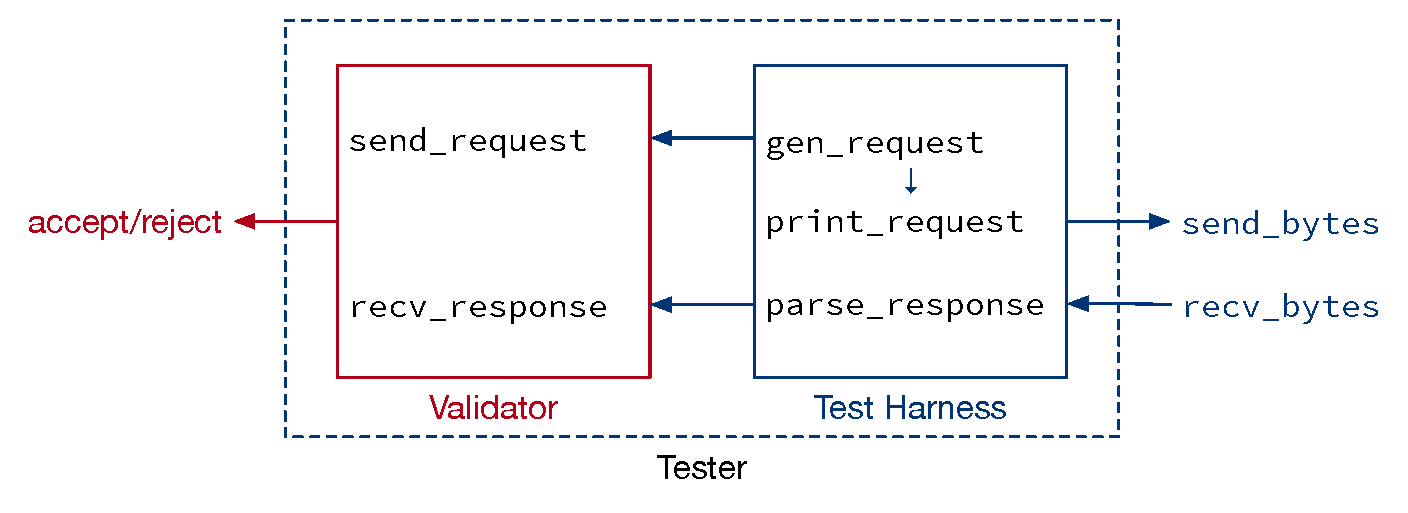
\includegraphics[width=.9\textwidth]{figures/harness-outline}
  \caption{Tester architecture outline.}
  \label{fig:overview}
\end{figure}

This section introduces the abstract architecture of an interactive tester,
using the networked server as an example.  I'll present a na\"ive implementation
of the test harness, which will be improved in the following sections.

The test harness interacts with the environment and provides the observations
for the validator.  The validator may represent requests and responses as
abstract datatypes for the convenience of specification.  The test harness
translates these abstract representations into bytes transmitted on the
underlying channel.

As shown in \autoref{fig:overview}, when the validator wants to observe a sent
request, the harness generates the request and encodes it into bytes to send.
Conversely, when the validator wants to observe a received response, the harness
receives bytes from the environment and decodes them into abstract messages.

\begin{figure}
\begin{lstlisting}[numbers=left]
Definition gen_packet: IO concrete_packet :=
  src          <- random_conn;;
  method       <- oneof [Get; Put];;
  target       <- random_path;;%\label{line:random-path}%
  precondition <- oneof [IfMatch, IfNoneMatch];;
  etag         <- random_etag;;
  payload      <- random_string;;
  ret { Source      := src;
        Destination := server_conn;
        Data        := inr { Method     := method;
                             TargetPath := target;
                             Headers    := [(precondition, etag)];
                             Payload    := payload
                           }
      }.
\end{lstlisting}
\caption{Na\"ive generator for HTTP requests.}
\label{fig:naive-generator}
\end{figure}

A generator is a randomized program that produces test inputs.  One example is
the \ilc{gen_packet} function in \autoref{fig:execute}.  The HTTP packet
generator can be na\"ively implementation as shown in
\autoref{fig:naive-generator}.  It fills in the request's fields with arbitrary
values, and has limited coverage of the SUT's behavior.  This is because the
request target and ETags are both generated randomly, but a request is
interesting only if its ETag matches its target's corresponding resource stored
on the server.  A randomly generated request would result in 404 Not Found and
412 Precondition Failed in almost all cases.

To reveal more interesting behavior from the SUT, we should tune the generator's
distribution to emphasize certain patterns of the test input.  For example, if
the tester knows the set of paths where the server has stored resources, then it
can generate more paths that correspond to existing resources; if the tester has
observed some ETags generated by the server, then it can include these ETags in
future requests.  In the next section, I'll explain how to implement such
heuristics in ITree-based testers.




As shown in \autoref{fig:overview}, the test framework consists of a {\em
  validator} that determines whether the SUT's behavior satisfies the
specification, and a {\em test harness} that provides test inputs for the
validator.

A {\em validator} is a client-side model program that observes messages sent and
received and decides whether these interactions are conformant to the
specification.  For example, a simple validator for echo server is written as:
\begin{lstlisting}[style=customcoq]
  let validateEcho =
    request := sendRequest();
    response := recvResponse();
    if response <> request
    then reject
    else validate
\end{lstlisting}
Notice that the \ilc{sendRequest} event does not take the request to be sent as
argument, but in stead returns the request actually sent.  The validator only
describes the logic that checks messages sent and received, while the test
harness computes what requests to send.

The {\em test harness} takes a validator and turns it into an executable program
that performs network interactions.  It handles the validator's send and receive
events, and generates the requests to be sent.  A simple test harness for the
validator above is written as:
\begin{lstlisting}[style=customcoq]
  let execute(v) =
    match v with
    | x := sendRequest(); v'(x) =>
      request := arbitraryRequest();
      sendBytes(print(request));
      execute(v'(request))
    | x := recvRequest(); v'(x) =>
      responseBytes := recvBytes();
      execute(v'(parse(responseBytes)))
    | reject => reject
    end in
  execute(validateEcho)
  (* ... is equivalent to ... *)
  let executeValidateEcho =
    request := arbitraryRequest();
    sendBytes(print(request));
    responseBytes := recvBytes();
    if parse(responseBytes) <> request
    then reject
    else executeValidateEcho
\end{lstlisting}

The \ilc{arbitraryRequest} generator here produces requests randomly.  To
generate requests that depend on previously observed messages, my framework will
extend the test harness in \autoref{fig:overview} that records a trace of
messages.

\section{Architecture}
\autoref{fig:shrink} shows the test harness architecture for networked
servers.  This framework involves four languages: (1) An {\em
  application representation} (AR) which provides flexible abstraction
for encoding the validation logic per protocol under test; (2) {\em
  Bytes} that the tester interacts with the SUT over network; between
them, (3) The {\em intermediate representation} (IR) for encoding the
trace in an application-independent way; and (4) The {\em symbolic
  representation} called ``J-expressions'' (Jexp) which encodes the
input generated and shrunk by the test harness.

\begin{figure}
  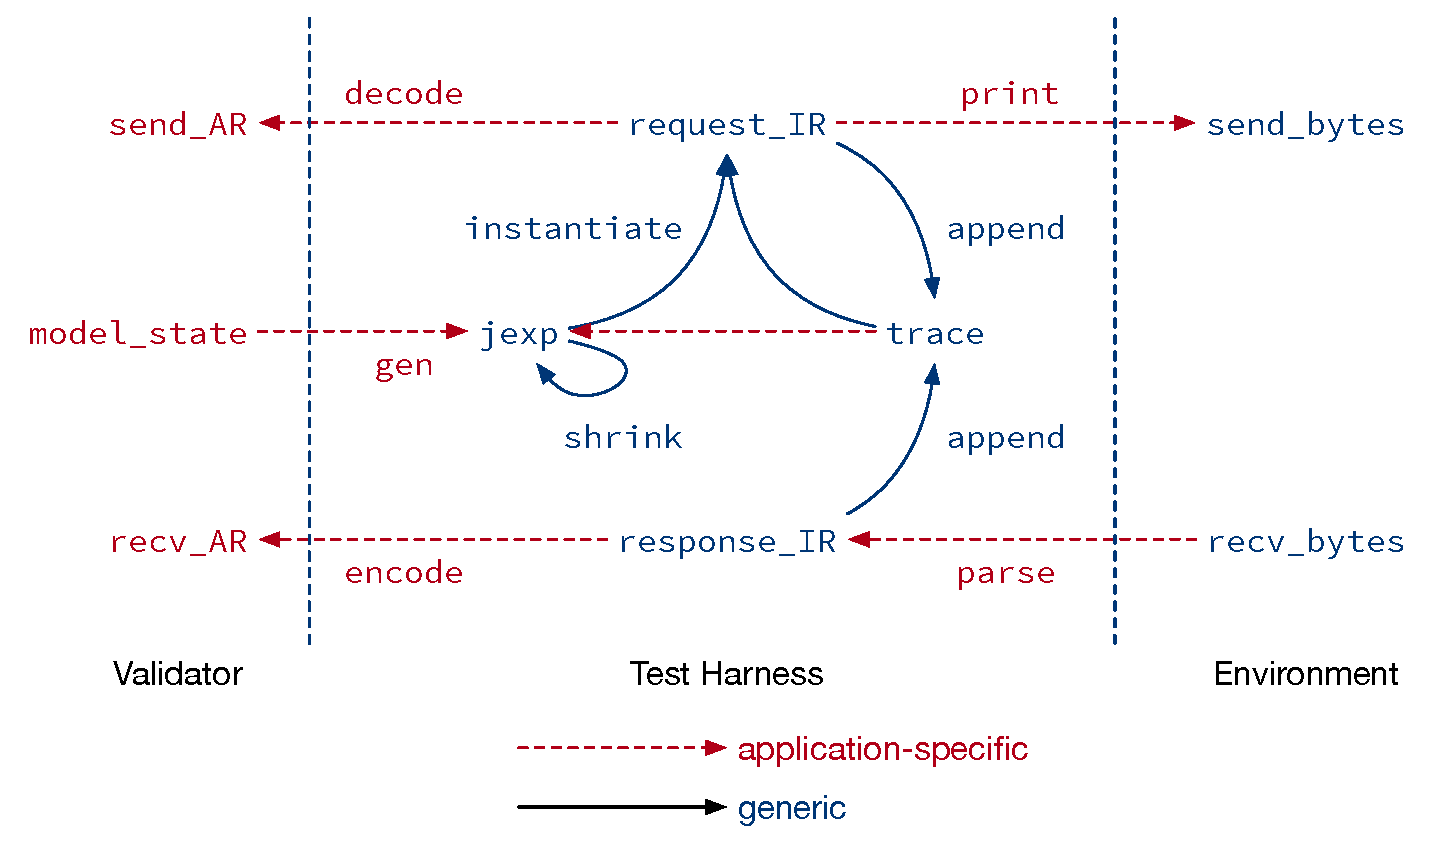
\includegraphics[width=.8\textwidth]{figures/shrink}
  \caption{Test harness architecture.  The test harness first generates
    J-expressions based on the model state provided by the validator.  The
    J-expression is a symbolic expressions that are instantiated by the trace
    into requests' IR.  When a violation is detected, the failing Jexp is shrunk
    into sub-expressions, and instantiated by the trace in new runs.  The dotted
    arrows are application-specific algorithms, while the solid arrows are
    generic over all protocols.}
  \label{fig:shrink}
\end{figure}

\section{Intermediate representation language}
The purpose of introducing an IR in this framework is to enable a generic method
for generating requests that refer to specific fields in the trace.  For
example, when testing conditional HTTP requests, the generator wants to include
``a precondition that uses the ETag field of a previous response''; when testing
an online store, the generator wants to provide ``an order ID that the server
has mentioned before''.

The IR in this framework is JSON, which allows syntax trees to be arbitrarily
wide and deep, and provides sufficient flexibility for network protocols in
general.  The J-expression is an extension of JSON that can refer to specific
fields in the trace:
\[\begin{array}{r@{\;}l}
\mathsf{JSON^T}\triangleq&\mathsf T\mid\{\mathsf{object^T}\}\mid[\mathsf{array^T}]\mid\mathsf{string}\mid\Nat\mid\Bool\mid\mathsf{null}\\
\mathsf{object^T}\triangleq&\nil\mid\mathsf{"string": JSON^T,object^T}\\
\mathsf{array^T}\triangleq&\nil\mid\mathsf{JSON^T,array^T}\\
\mathsf{IR}\triangleq&\mathsf{JSON^{IR}}\\
\mathsf{Jexp}\triangleq&\mathsf{JSON^{\Jref{\mathit{label}}{\mathsf{Jpath}}{\mathit{function}}}}\\
&\text{where }\mathit{label}\in\Nat,\mathit{function}\in\mathsf{IR}\to\mathsf{IR}\\
\Jpath\triangleq&\This\mid\Jpath\Number\mathit{index}\mid\Jpath\At\mathit{field}\\
&\text{where }\mathit{index}\in\Nat,\mathit{field}\in\mathsf{string}
\end{array}\]

The extended syntax
``$\Jref{\mathit{label}}{\mathsf{Jpath}}{\mathit{function}}$'' is a symbolic
expression that, given a runtime trace, can compute an IR of the request.  For
example, J-expression
``$\Jref{3}{\This\At\mathtt{"orders"}\Number2}{\mathtt{id}}$'' can be
pronounced: ``Look at the message labelled 3 in the trace, its `order' field
should be an array.  Find the 2nd element in that array, and use it
\ilc{id}entically (as-is).''  Such representation enables the test harness to
shrink counterexamples (encoded in Jexp) in a protocol-independent way.


\begin{figure}
  \begin{lstlisting}[style=customcoq]
    Example response1 : http_response :=
      Response (Status (Version 1 1) 200 (Some "OK"))
               [Field "ETag" "tag-foo";
                Field "Content-Length" "11"]
               (Some "content-bar").

    Example response2 : store_response :=
      Response__ListOrders [(233, (12, 100, 34, 500));
                            (996, (56, 400, 78, 20))].
  \end{lstlisting}
  \begin{minipage}[t]{.4\textwidth}
    \begin{lstlisting}[style=json]
      {
        "version": {
          "major": 1,
          "minor": 1
        },
        "code": 200,
        "reason": "OK",
        "fields": {
          "ETag": "tag-foo",
          "Content-Length": "11"
        },
        "body": "content-bar"
      }
    \end{lstlisting}
  \end{minipage}%
  \begin{minipage}[t]{.4\textwidth}
    \begin{lstlisting}[style=json]
      {
        "code": 200,
        "orders": [
          {
            "ID": 233,
            "BuyerID": 12,
            "BuyAmount": 100,
            "SellerID": 34,
            "SellAmount": 500
          },
          {
            "ID": 996,
            "BuyerID": 56,
            "BuyAmount": 400,
            "SellerID": 78,
            "SellAmount": 20
          }
        ]
      }
    \end{lstlisting}
  \end{minipage}
  \caption{Application message example for HTTP and online store protocols, and
    their corresponding intermediate representation}
  \label{fig:ir}
\end{figure}

To represent the correspondence between requests and responses, the trace labels
each message, and the request-response pair have the same label.
\autoref{fig:trace} shows a trace of messages sent and received by the tester
client.

\begin{figure}
  \begin{minipage}{.5\textwidth}
    \begin{lstlisting}[style=json]
      [
        {
          "label": 10,
          "message": {
            "method": "GET",
            "path": "index.html"
          }
        },
        {
          "label": 20,
          "message": {
            "method": "DELETE",
            "path": "index.html"
          }
        },
        {
          "label": 20,
          "message": {
            "code": 204,
            "reason": "No Content",
          }
        },
        {
          "label": 10,
          "message": {
            "code": 410,
            "reason": "Gone"
          }
        }
      ]
    \end{lstlisting}
  \end{minipage}%
  \begin{minipage}{.5\textwidth}
    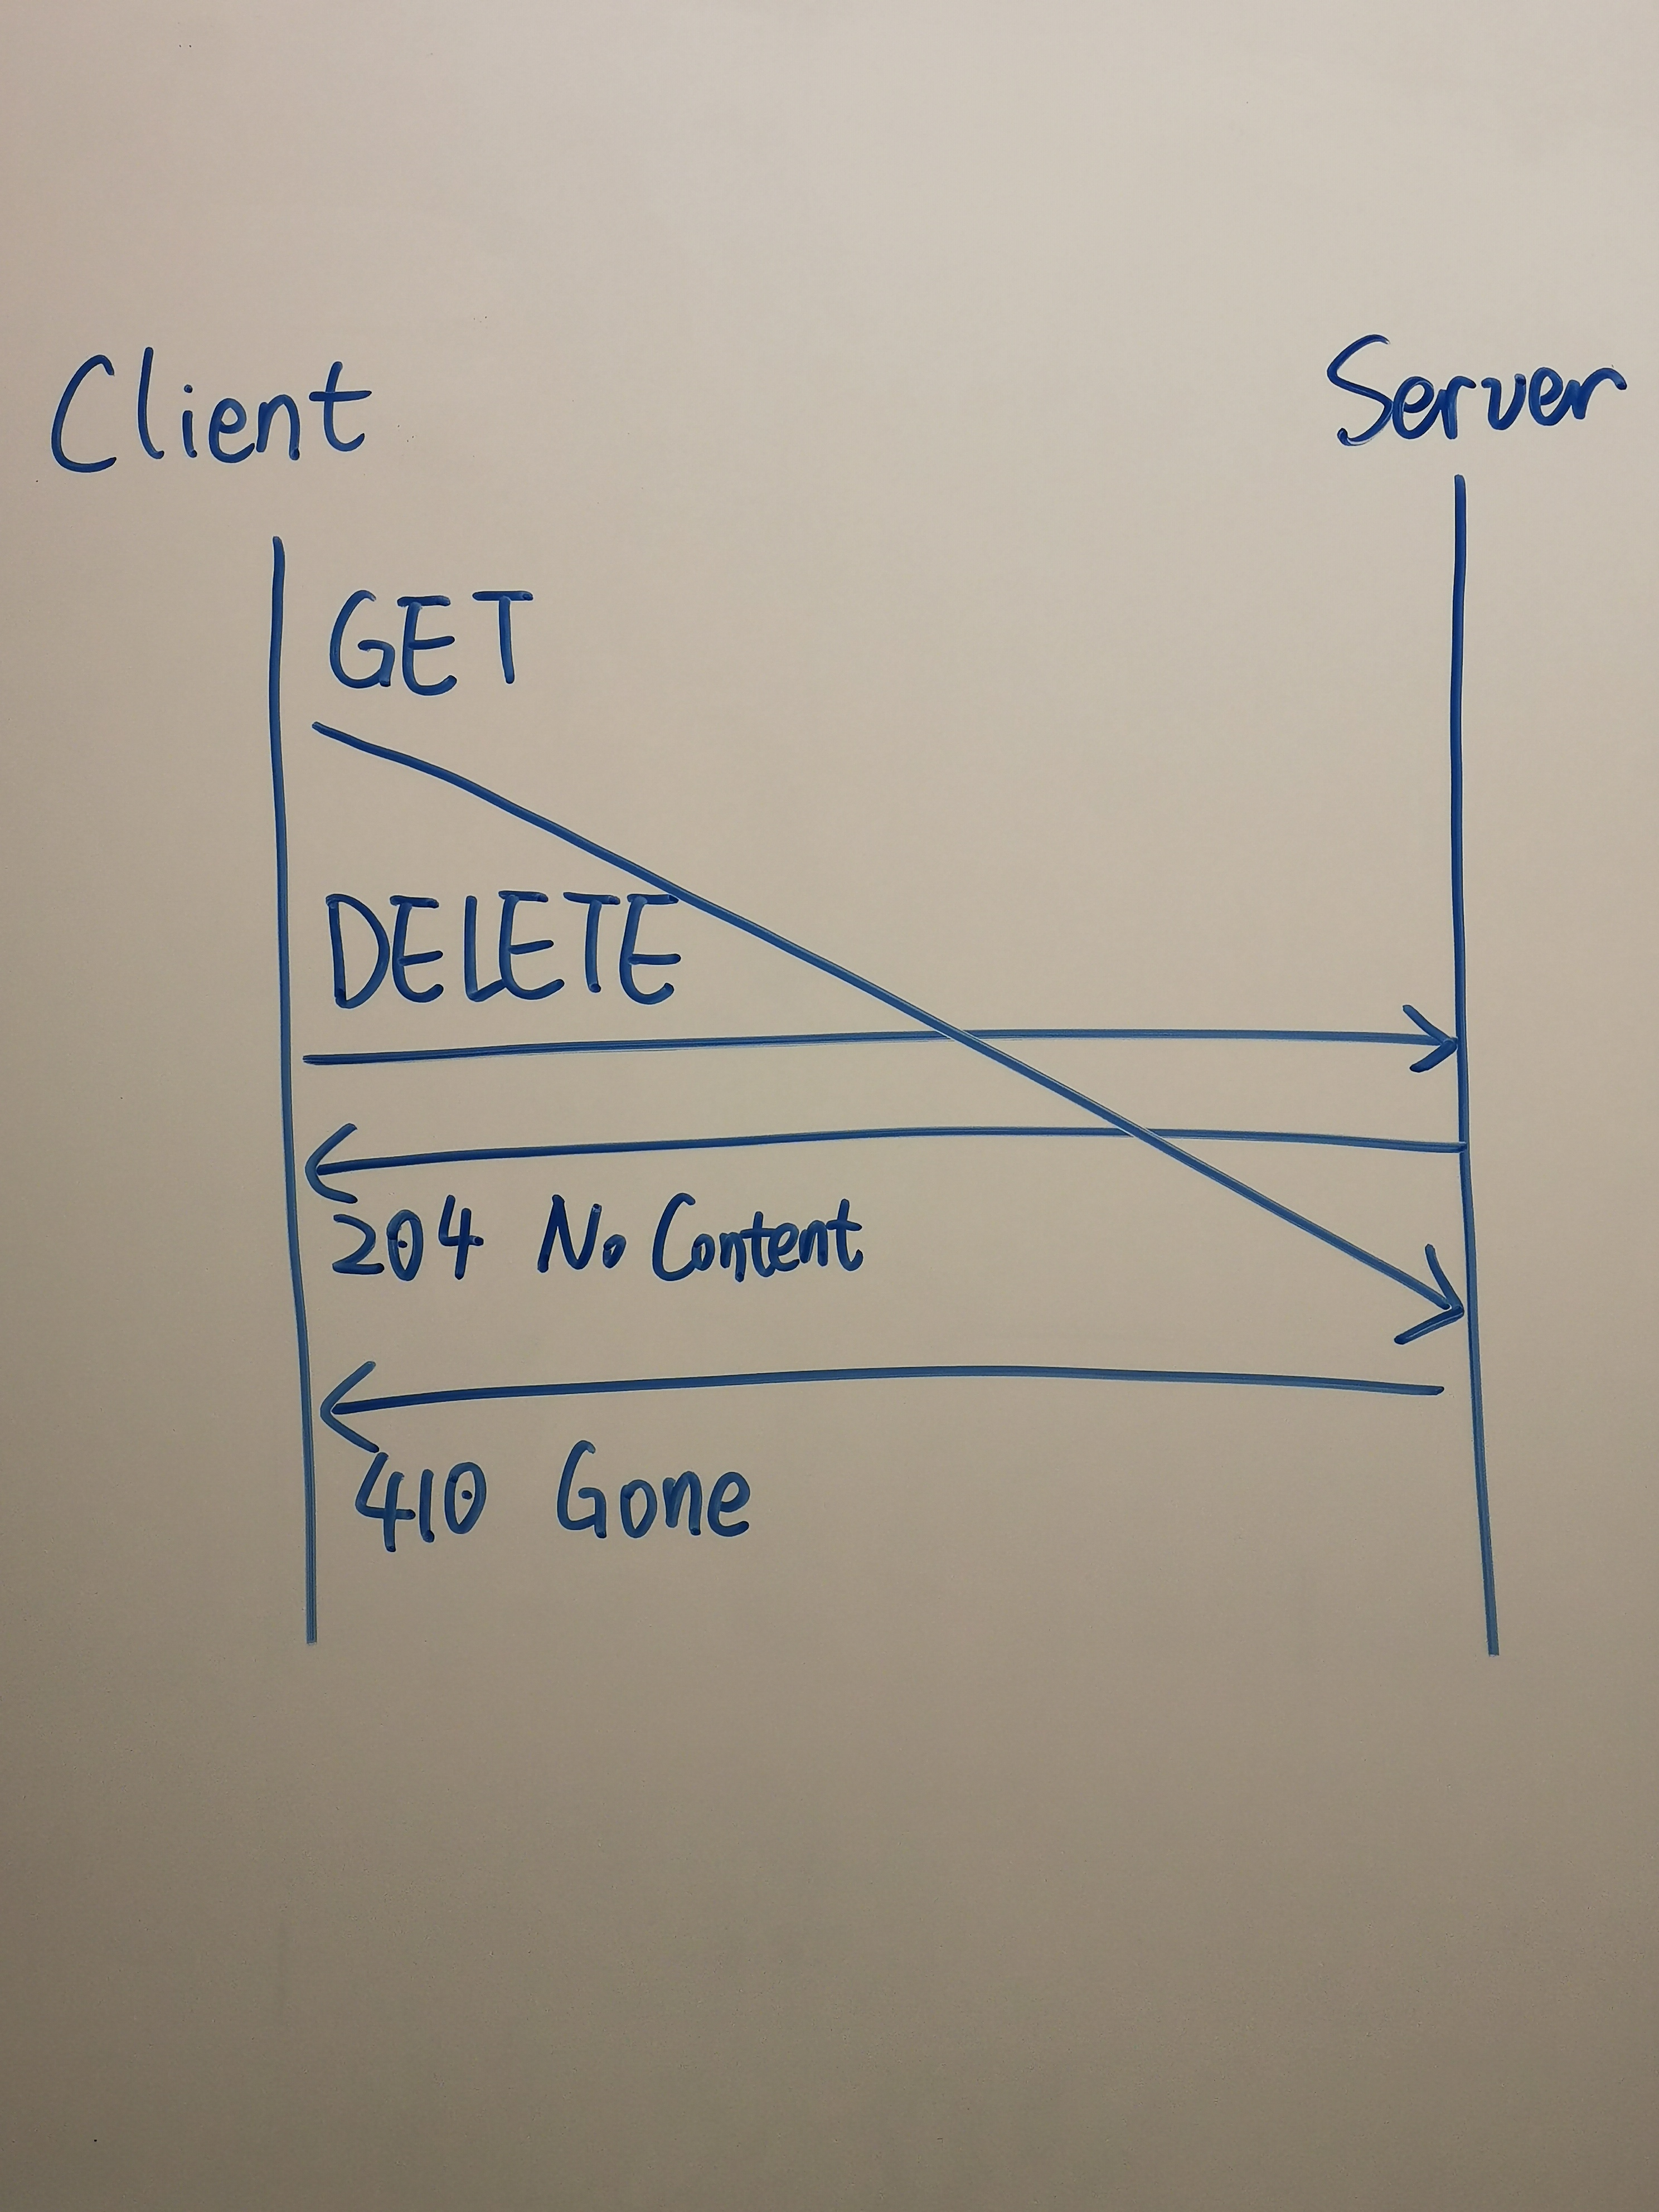
\includegraphics[width=\textwidth]{figures/trace}
  \end{minipage}
  \caption{Example client-side trace and its corresponding IR}
  \label{fig:trace}
\end{figure}

\section{Instantiating requests during runtime}
To instantiate a Jexp into request IR, the test harness substitutes all
occurences of ``$\Jref{\mathit{label}}{\mathsf{Jpath}}{\mathit{function}}$''
with its corresponding IR computed from the trace.  However, due to external
nondeterminism, the expected message label might be delayed and not available in
the trace.  Also, considering inter-execution nondeterminism, arrays in observed
messages might not have enough elements as expected in the Jexp.  In these
cases, the test harness searches for other labels in the trace and other
elements in the arrays as a fallback fulfillment to construct the request.

\lys{Todo: add instantiation algorithm.}

This idea of shrinking symbolic representations can be applied to scenarios
beyond networked servers.  For example, the HTTP testing experiment in
\autoref{sec:eval} has also used this technique to locate the bug pattern.
